\documentclass{report}

\usepackage{amsmath}
\usepackage{geometry}
\usepackage{amsfonts}
\usepackage[english]{babel}
\usepackage{amssymb}
\usepackage{graphicx}
\usepackage{float}
\usepackage{hyperref}
\usepackage{multirow}
\usepackage{pdflscape}
\usepackage{caption}
\usepackage{pdflscape}
\usepackage{outlines}
\usepackage{subcaption}
\usepackage{enumerate}
\usepackage[latin1]{inputenc}

\usepackage{tabularx, booktabs}
\usepackage{longtable}

\usepackage{standalone}

\usepackage[autostyle, english = american]{csquotes}
\MakeOuterQuote{"}

\usepackage{comment}

\newcommand{\tabnotes}[2]{\bottomrule \multicolumn{#1}{@{}p{0.95\linewidth}@{}}{\footnotesize #2 }\end{tabular}\end{table}}

\title{PCR and Measurement Error}
\author{Isaac Liu}
\date{\today}

\setlength{\parindent}{0pt}
\setlength{\parskip}{0.5em}

\hypersetup{
    colorlinks=true,
    linkcolor=blue,
    filecolor=magenta,      
    urlcolor=cyan,
}

\begin{document}

	\maketitle

	\newpage \clearpage

    \section*{Application: GDP and Life Expectancy}

	% Add \ref to the following table?
	In the left column in the table below I first regress the life expectancy at birth for all individuals in a given country and year on the World Bank's PPP adjusted GDP per capita. In the right column I regress the same life expectancy measure on the first principal component combining GDP per capita (PPP), GNI per capita (PPP), Survey Mean Income/Consumption Per Capita, ILO GDP per person employed, and Net Foreign Assets Per Capita, all from the World Bank.
	
	I standardize all variables by subtracting the mean and dividing by the standard deviation, linearly interpolate data between known observations, and remove country-years with missing values for any of the economic indicators.

    \begin{table}[!htbp] \centering
\begin{tabular}{@{\extracolsep{5pt}}lcc}
\\[-1.8ex]\hline
\hline \\[-1.8ex]
& \multicolumn{2}{c}{\textit{Life Expectancy at Birth}} \
\cr \cline{2-3}
\\[-1.8ex] & (1) & (2) \\
\hline \\[-1.8ex]
 GDP Per Capita, PPP & 0.002$^{***}$ & \\
  & (0.000) & \\
 Estimated Factor & & 0.000$^{***}$ \\
  & & (0.000) \\
\hline \\[-1.8ex]
 Observations & 11,708 & 11,708 \\
 $R^2$ & 0.485 & 0.005 \\
 Adjusted $R^2$ & 0.485 & 0.005 \\
 Residual Std. Error & 46.966 & 65.300  \\
 F Statistic & 11036.059$^{***}$  & 58.084$^{***}$  \\
\hline
\hline \\[-1.8ex]
\textit{Note:} & \multicolumn{2}{r}{$^{*}$p$<$0.1; $^{**}$p$<$0.05; $^{***}$p$<$0.01} \\
\end{tabular}
\end{table}

	Though the coefficients are not readily interpretable, they do differ from each other

	ADD TEST to show coefficients differ? I think this also would not be easy to interpret since the independent variables are different...

	In both cases, they are significant.
	
	Notably, we demonstrate a higher $R^2$ using the principal component model.

    \clearpage \newpage

    \appendix

    \section*{Appendix}

	\begin{figure}[h!]
		\centering
		\caption{Correlations Between Economic Measures and Life Expectancy}
		\label{GDP_LE_Correlations_Correlations}	
		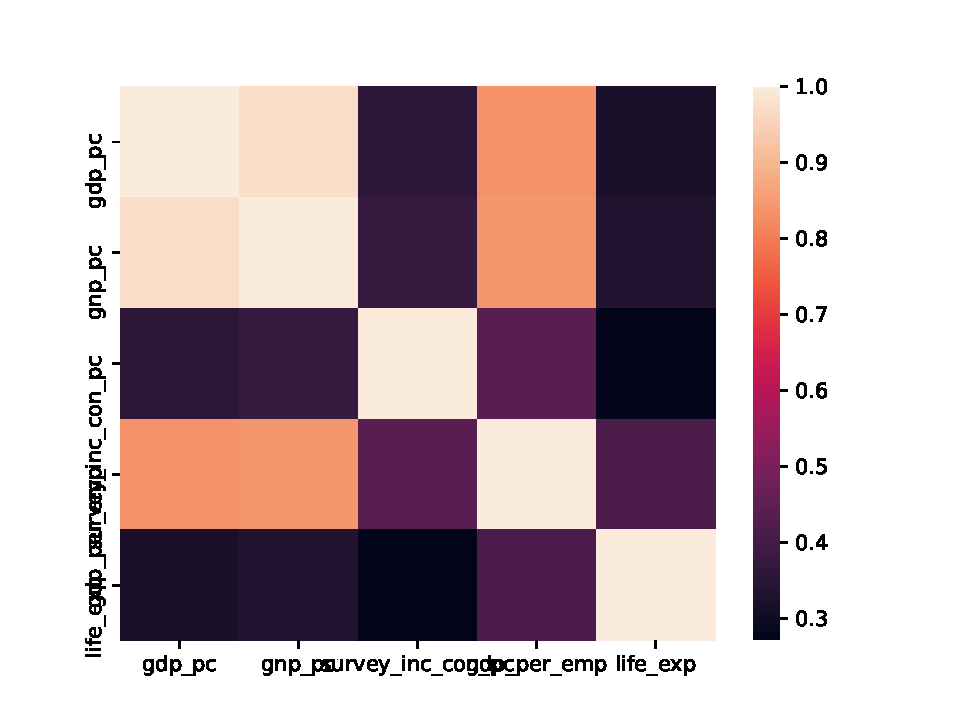
\includegraphics[width=\linewidth,keepaspectratio=true]{../Output/Figures/GDP_LE_Correlations.pdf}
	\end{figure}

	\begin{figure}[h!]
		\centering
		\caption{Economic Measures PCA Loadings}
		\label{Econ_Loadings}	
		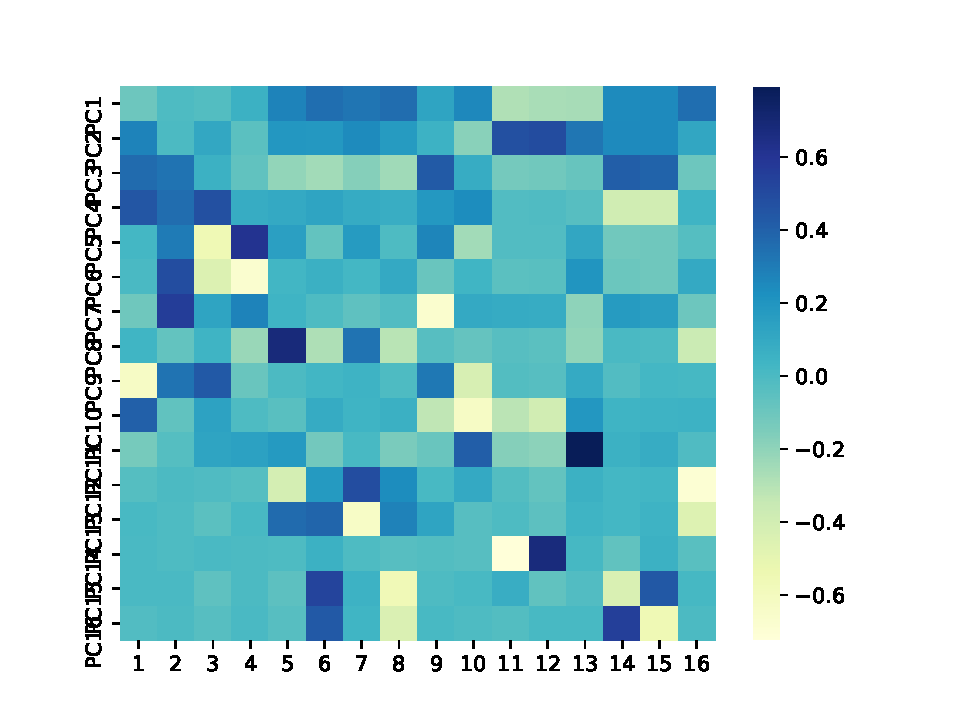
\includegraphics[width=\linewidth,keepaspectratio=true]{../Output/Figures/GDP_LE_Loadings.pdf}
	\end{figure}

	\begin{figure}[h!]
		\centering
		\caption{Economic Measures PCA Share of Variance Explained}
		\label{Econ_Share_Explained}	
		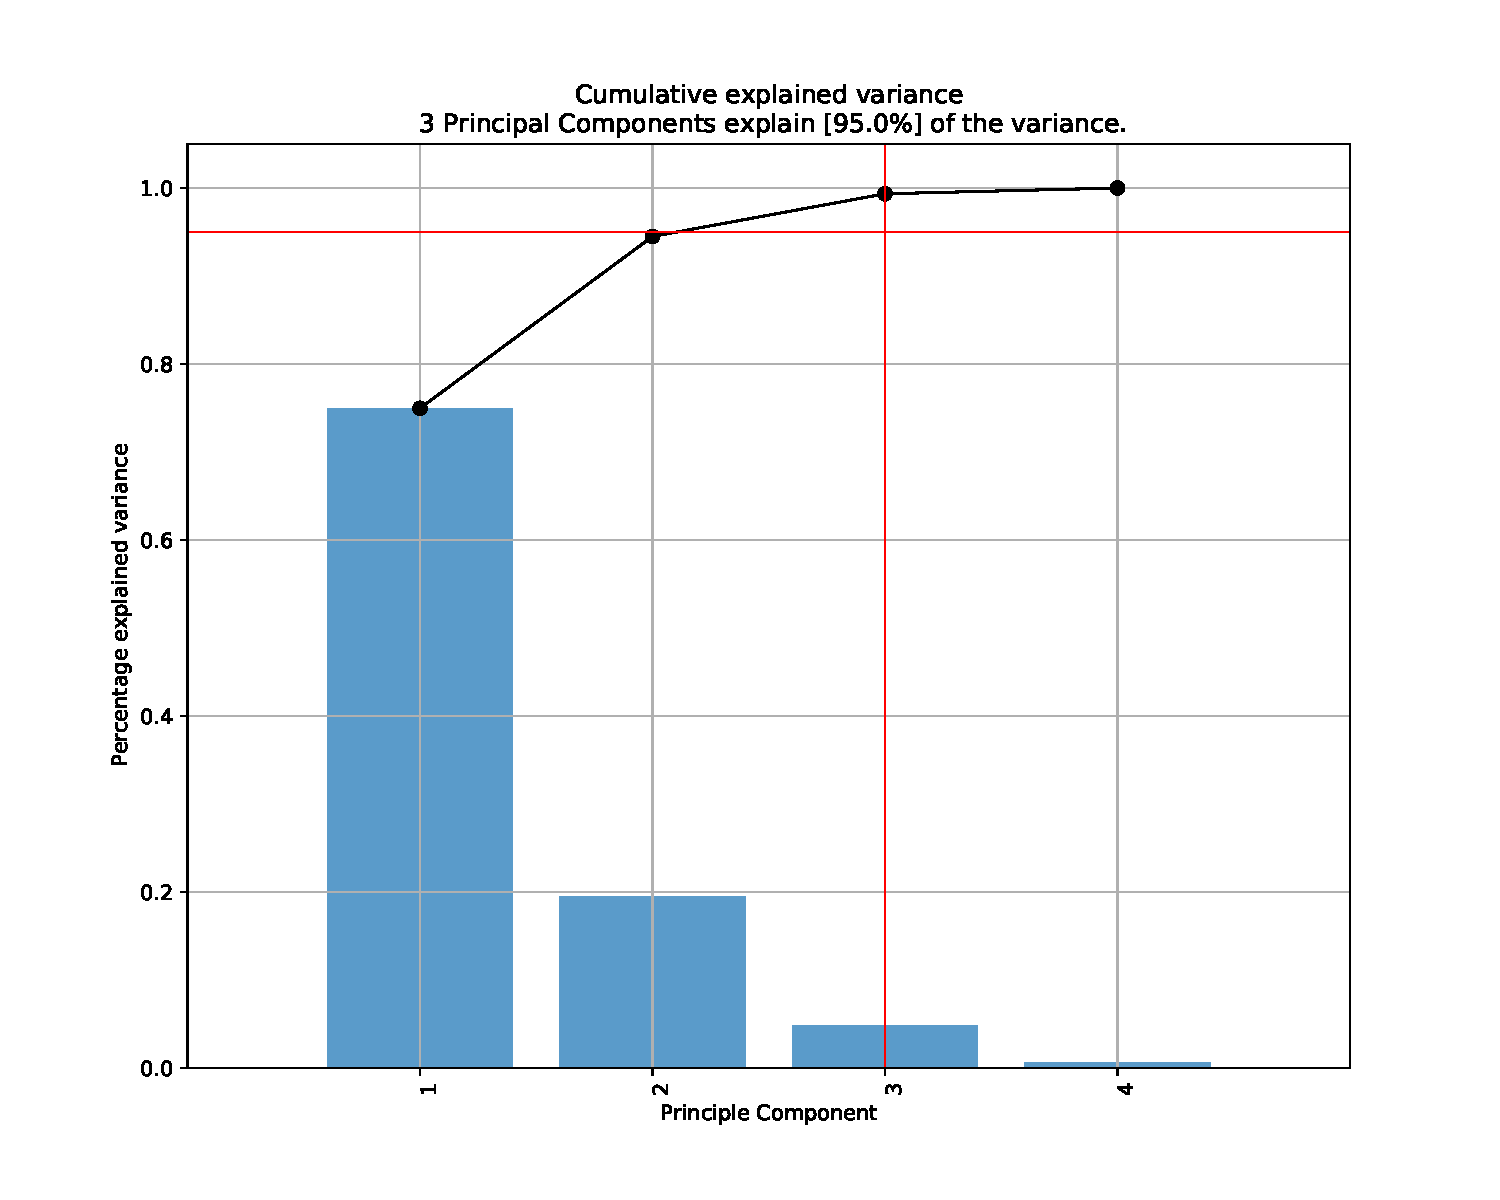
\includegraphics[width=\linewidth,keepaspectratio=true]{../Output/Figures/GDP_LE_Share_Explained.pdf}
	\end{figure}

\end{document}